\section{Supplement}
All analysis code is available online at:
\hreftt{github.com/mishra-lab/duration-bias}
%===================================================================================================
\subsection{Beta Approximation of the Binomial Distribution}\label{app.bab}
The distributions of RDS-adjusted variables in \cite{Baral2014} were reported as
frequency tables with variable values and adjusted proportions (mean, \ci).
For each proportion, we defined a beta approximation of the binomial (BAB) distribution:
\begin{alignat}{1}\label{eq:bab}
  p(\rho) &=
    \frac{\Gamma(\alpha+\beta)}{\Gamma(\alpha)\,\Gamma(\beta)}\,
    \rho^{\alpha-1}{(1 - \rho)}^{\beta-1} \\
    &\approx {N \choose n} \, \rho^{n}{(1 - \rho)}^{N - n} \nonumber
\end{alignat}
with $\alpha = N\,\rho$ and $\beta = N\,(1-\rho)$.
We fixed $\rho$ as the adjusted point estimate,
and estimated $N$ by minimizing the sum of squared differences between
the 95\% quantiles of \eqref{eq:bab} given $N$ and the reported \ci for the adjusted proportion.
%===================================================================================================
\subsection{Risk Group Duration}\label{app.yss}
%---------------------------------------------------------------------------------------------------
\paragraph{Fitted Exponential}
We fit an exponential distribution (\ie estimated $\lambda$) to the RDS-adjusted proportions for
``years selling sex'' in \cite{Baral2014} by
maximizing the overall likelihood (product of individual likelihoods) across BAB distributions,
where each proportion was defined as:
\begin{equation}
  \rho_i = F(t_i) - F(t_{i-1}), \quad F(t) = 1 - e^{-\lambda t}
\end{equation}
Figure~\ref{fig:yss.fit} illustrates the resulting cumulative distribution \vs
the target cumulative proportions.
\begin{figure}[h]
	\centering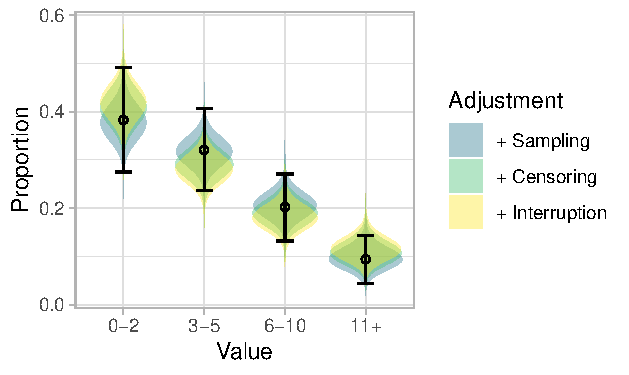
\includegraphics[scale=.8]{yss.fit}
  \caption{Estimated cumulative exponential distribution for years selling sex,
    fitted to RDS-adjusted proportions}
	\label{fig:yss.fit}
  \floatfoot{Guide:
    \g{circles}{mean adjusted cumulative proportions $\rho_i$ selling sex for $y_i$ years},
    \g{bars}{\ci for $\rho_i$},
    \g{line}{exponential distributon estimate},
    \g{shaded ribbon}{\ci}.
    Data from \cite{Baral2014}}
\end{figure}
%---------------------------------------------------------------------------------------------------
\paragraph{Numeric Summary}
Table~\ref{tab:yss.adj} summarizes the estimated exponential distribution means (\ci)
for years selling sex following each stage of adjustment outlined in \sref{meth.yss}.
\begin{table}[h]
  \centering
  \caption{Estimated mean durations selling sex (years) following each stage of adjustment}
  \begin{tabular}{lrc}
  \toprule
  Adjustment     & Mean & (\ci) \\
  \midrule
  Median         & 4.00 & --- \\
  Mean           & 5.77 & --- \\
  + Sampling     & 4.35 & (3.27,~\w5.72) \\
  + Censoring    & 9.40 & (6.60,~13.22) \\
  + Interruption & 4.06 & (2.29,~\w6.34) \\
  \bottomrule
\end{tabular}

  \label{tab:yss.adj}
  \floatfoot{Data from \cite{Baral2014}.}
\end{table}
%===================================================================================================
\subsection{Rate of Partnership Change}\label{app.partners}
%---------------------------------------------------------------------------------------------------
\paragraph{Mean Reported Partners}
We repeated the following for each partnership type
(new paying clients, regular paying clients, and non-paying partners).
We estimated the mean number of reported partners $\bar{x}$ as a weighted average
of the reported partners $x_i$ with the RDS-adjusted proportions $\rho_i$:
\begin{equation}\label{eq:x.bar}
  \bar{x} = \sum\nolimits_i \rho_i x_i
\end{equation}
To capture uncertainty in the proportions $\rho_i$,
we fitted a BAB distribution (\ie estimated $N_i$) in each case, as described in \sref{app.bab}.
Then, we randomly sampled sets of $\rho$,
normalized these sets by the sum (such that $\sum_i \rho_i = 1$), and
re-calculated $\bar{x}$ for each set.
Figure~\ref{fig:partners.fit} illustrates
the resulting uncertainty distributions for $\bar{x}$,
along with the corresponding $x_i$.
\begin{figure}[h]
  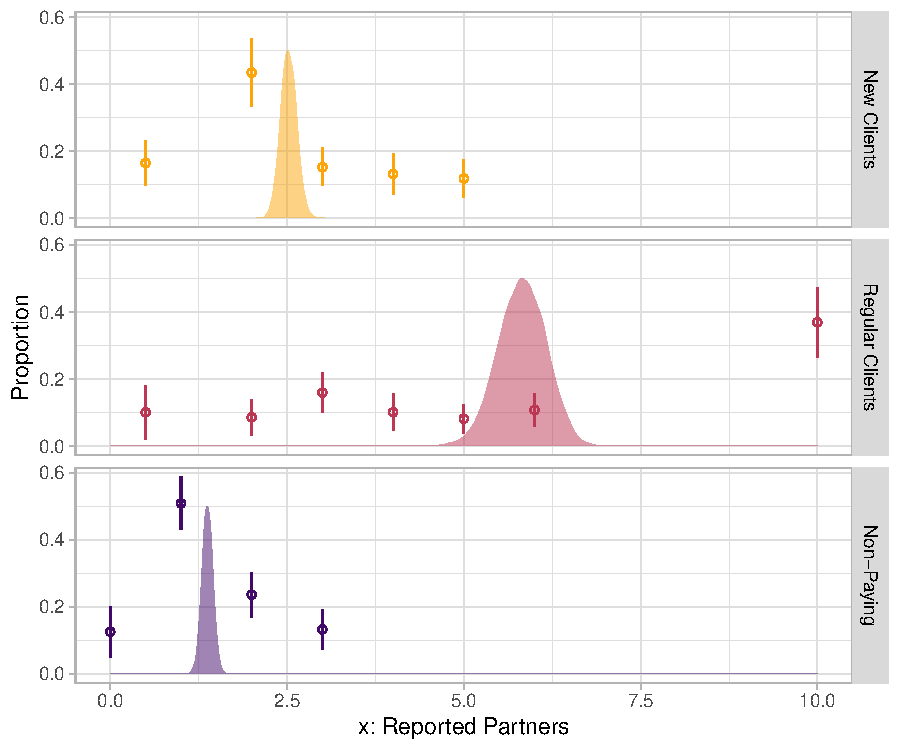
\includegraphics[width=\textwidth]{partners.fit}
  \caption{Distributions of numbers of reported partners in the past 30 days}
  \label{fig:partners.fit}
  \floatfoot{Guide:
    \g{circles}{mean adjusted proportions $\rho_i$ reporting $x_i$ partners},
    \g{bars}{\ci for $\rho_i$},
    \g{shaded area}{empiric distribution of $\bar{x}$}.
    Data from \cite{Baral2014}.}
\end{figure}
\begin{table}[h]
  \centering
  \caption{Biased \vs unbiased estimates of
    rates of partnership change and numbers of current partners
    for three partnership types reported by female sex workers}
  \begin{tabular}{llrcrc}
  \toprule
   & & \multicolumn{2}{c}{Rate $Q$} &
       \multicolumn{2}{c}{Number $K$} \\
  \cmidrule(rl){3-4}\cmidrule(rl){5-6}
  Partnership Type & Bias & Mean & 95\%~CI & Mean & 95\%~CI \\
  \midrule
  New Clients     & Biased   & 1.77 & (1.65,\,1.89) & 1.77 & (1.65,\,1.89) \\
                  & Unbiased & 1.71 & (1.60,\,1.83) & 0.06 & (0.05,\,0.06) \\
  Regular Clients & Biased   & 4.69 & (4.49,\,4.89) & 4.69 & (4.49,\,4.89) \\
                  & Unbiased & 0.94 & (0.90,\,0.98) & 3.75 & (3.60,\,3.91) \\
  Non-Paying      & Biased   & 0.74 & (0.66,\,0.82) & 0.74 & (0.66,\,0.82) \\
                  & Unbiased & 0.02 & (0.02,\,0.02) & 0.72 & (0.64,\,0.80) \\
  \bottomrule
\end{tabular}

  \label{tab:partners.fsw}
  \floatfoot{Rares are per-month. Data from \cite{Baral2014}.}
\end{table}
